%%
% Please see https://bitbucket.org/rivanvx/beamer/wiki/Home for obtaining beamer.
%%
\documentclass{beamer}

\usetheme{Luebeck}
\usecolortheme{crane}
\setbeamertemplate{section in toc}[ball unnumbered]
\setbeamertemplate{subsection in toc}[ball unnumbered]

\usepackage[T1]{fontenc}
\usepackage{beramono}
\usepackage{graphicx}
\usepackage{hyperref}
\usepackage{pifont}
\usepackage{listings}
\usepackage{xcolor}
\usepackage{multicol}


%\definecolor{darkgreen}{rgb}{0.,0.6,0.}

\newcounter{questionizeIndex}

\newenvironment{questionize}[1][0]{%
    \setbeamercovered{invisible}%
    \setcounter{questionizeIndex}{#1}%
    \begin{itemize}%
}{ %
    \end{itemize}%
}

\newcommand{\question}[2]{%
    % #1: question
    % #2: answer (replaces question)
    \stepcounter{questionizeIndex}%
    \item<\value{questionizeIndex}->%
    \only<\value{questionizeIndex}>{#1}%
    \stepcounter{questionizeIndex}%
    \only<\value{questionizeIndex}->{#2}%
}

\newcommand{\lquestion}[4]{%
    % #1: question label
    % #2: question
    % #3: answer label
    % #4: answer (replaces question)
    \stepcounter{questionizeIndex}%
    \item[\only<\value{questionizeIndex}->{\alt<\value{questionizeIndex}>{#1}{#3}}]<\value{questionizeIndex}->%
    \only<\value{questionizeIndex}>{#2}%
    \stepcounter{questionizeIndex}%
    \only<\value{questionizeIndex}->{#4}%
}

\newcommand{\cquestion}[2]{\question{#2}{\color{#1}{#2}}}

\newcommand{\ctrue}[1]{\cquestion{darkgreen}{#1}}
\newcommand{\cfalse}[1]{\cquestion{red}{#1}}

\newcommand{\ltrue}[1]{\lquestion{\textbf{?}}{#1}{$\checkmark$}{#1}}
\newcommand{\lfalse}[1]{\lquestion{\textbf{?}}{#1}{$\times$}{#1}}

\lstset{
    basicstyle=\footnotesize\ttfamily,
    breaklines=true
}


\hypersetup{%
  colorlinks=true,% hyperlinks will be black
  pdfborderstyle={/S/U/W 1}% border style will be underline of width 1pt
}
\begin{document}

\title{MSiA490 SEC20/28\\ Text Analytics}
\subtitle{Lab 2 - Word2Vec}
\author{Timo Wang}
\institute{Northwestern University}
\date{September 24th, 2020 \\
{\footnotesize Some slides of this document is built based on the content provided on https://github.com/tmikolov/word2vec.}}

\begin{frame}
    \titlepage
\end{frame}

%\begin{frame}{Overview}
%    \tableofcontents[hideallsubsections]
%\end{frame}

\section{What is Word2Vec?}
\begin{frame}
    \frametitle{What is Word2Vec?}
    \begin{figure}
        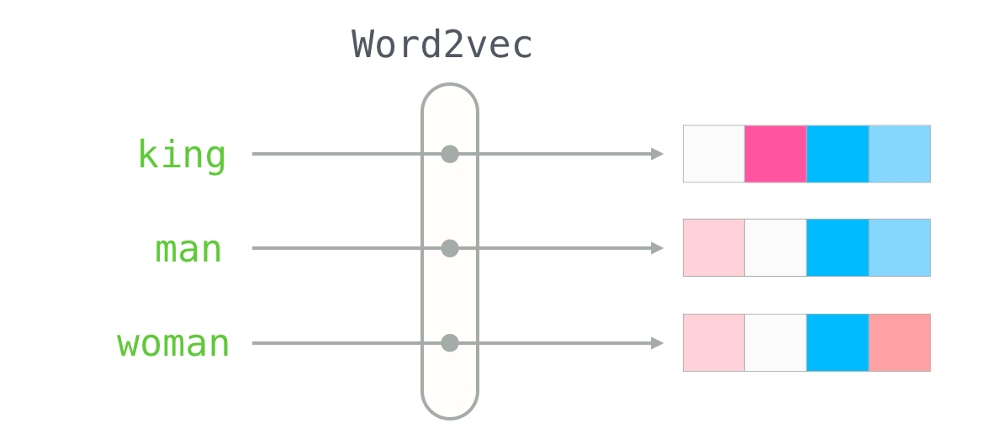
\includegraphics[scale=0.5]{what-is-word2vec}
        \caption{It encodes a word into a vector, in comparison to one-hot encoder, where each word is represented by an integer.}
    \end{figure}
\end{frame}


\section{Why do we care?}
\begin{frame}
    \frametitle{Why do we care?}
    \framesubtitle{Better capture of word meaning}
    \begin{figure}
        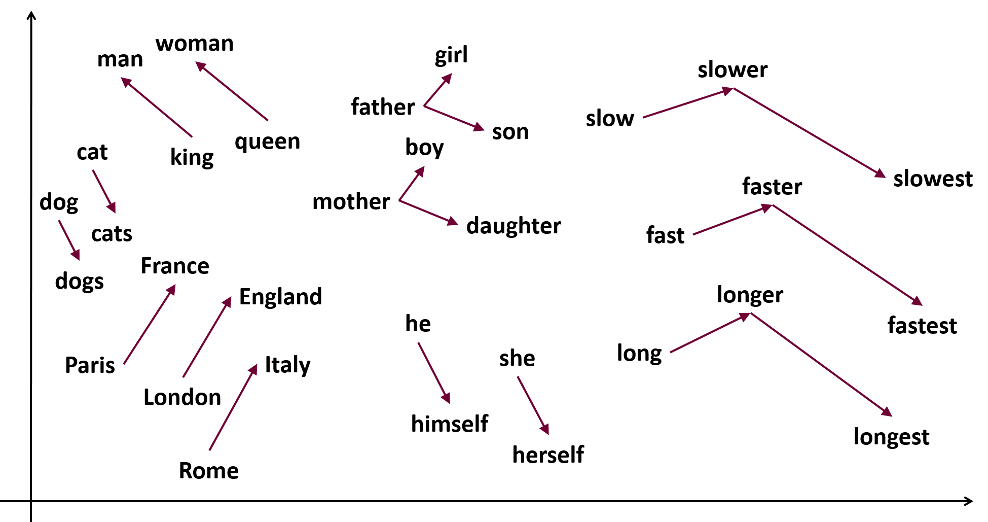
\includegraphics[scale=0.5]{why-word2vec-1}
    \end{figure}
\end{frame}

\section{How does it work?}
\begin{frame}
    \frametitle{How does it work?}
    \begin{figure}
        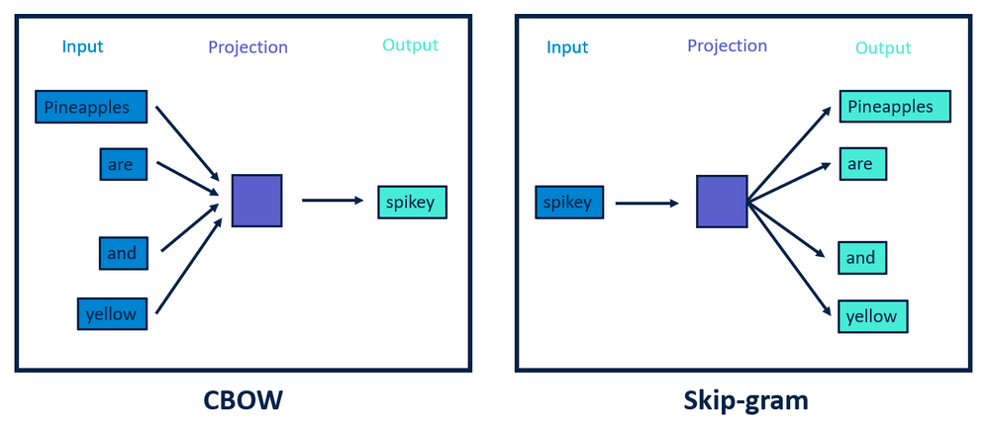
\includegraphics[scale=0.5]{how-word2vec-works}
    \end{figure}
\end{frame}

\section{How well does it perform?}
\subsection{Strength}
\begin{frame}
    \frametitle{How well does it perform?}
    \framesubtitle{Strength}
    \begin{figure}
        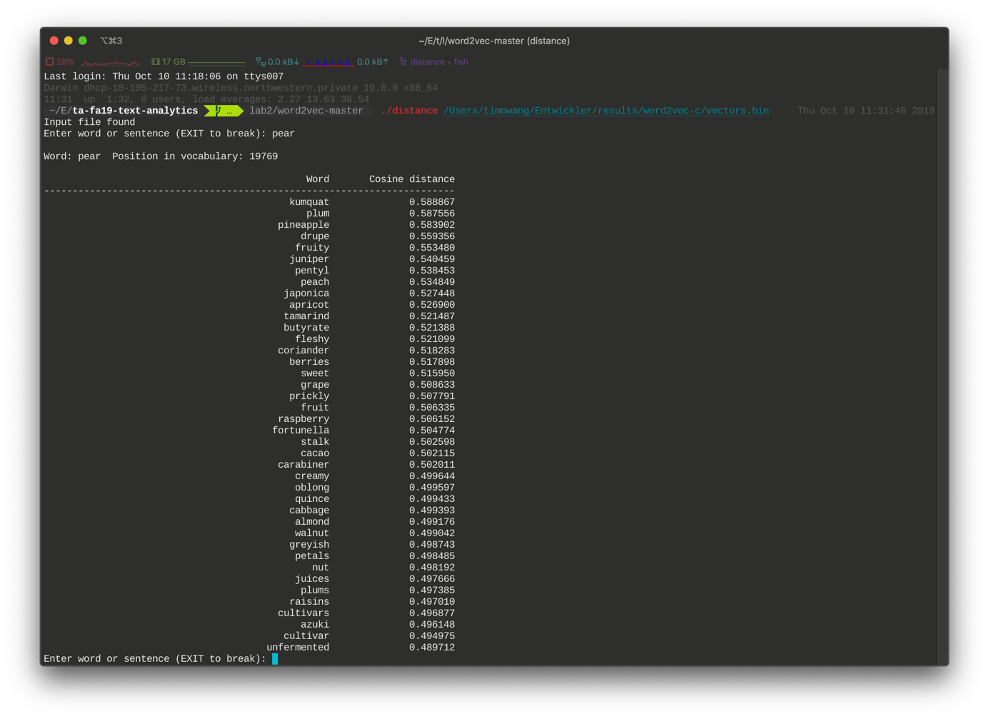
\includegraphics[scale=0.45]{strength}
    \end{figure}
\end{frame}

\subsection{Weakness}
\begin{frame}
    \frametitle{How well does it perform?}
    \framesubtitle{Weakness}
    \begin{figure}
        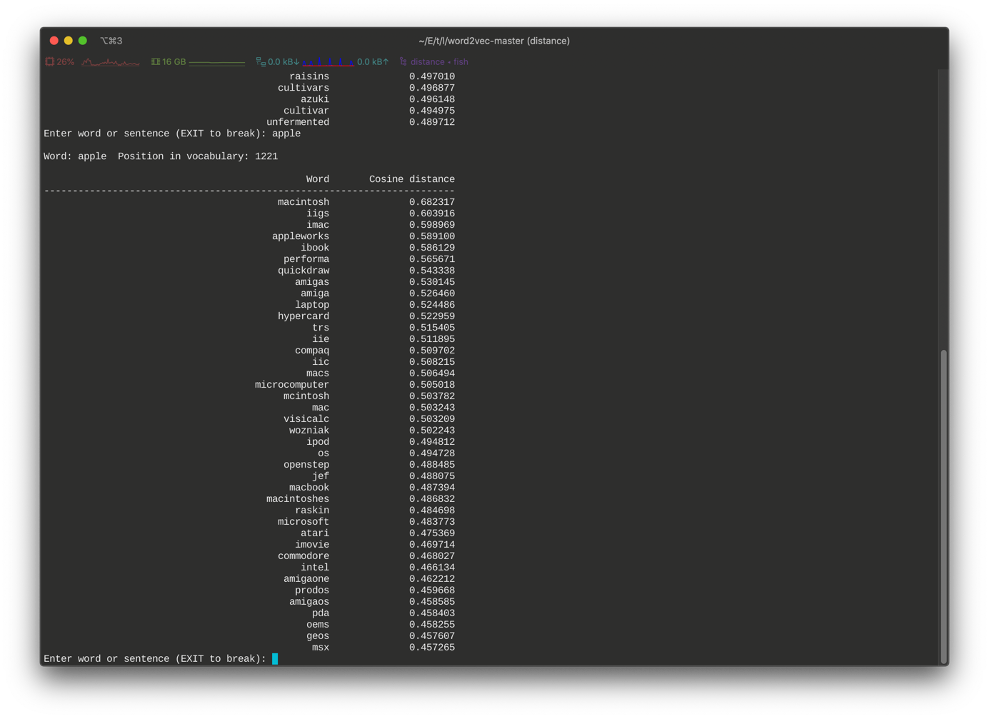
\includegraphics[scale=0.45]{weakness}
    \end{figure}
\end{frame}

\section{Tools \& libraries}

\subsection{Demo}
\begin{frame}[containsverbatim]
    \frametitle{Tools \& libraries}
    \framesubtitle{Demo}
    \begin{block}{Shell}
        \scriptsize
        \begin{lstlisting}
# Download and decompress a sample text corpus.
wget http://mattmahoney.net/dc/text8.zip -O text8.gz
tar xvf text8.gz

# Train a model named vectors.bin with the downloaded corpus text8
./word2vec -train text8 -output vectors.bin -cbow 1 -size 200 -window 8 -negative 25 -hs 0 -sample 1e-4 -threads 20 -binary 1 -iter 15
# Examine the embedding
./distance vectors.bin
        \end{lstlisting}
    \end{block}
\end{frame}


\subsection{The original library}
\begin{frame}
    \frametitle{Tools \& libraries}
    \framesubtitle{The original library}
    \begin{enumerate}
        \item[Step 1] Download the project from \href{https://github.com/tmikolov/word2vec}{https://github.com/tmikolov/word2vec}.
        \item[Step 2] Read \texttt{demo-word.sh}.
        \item[Step 3] Use \texttt{demo-word.sh} as a guideline and train the model with your own corpus. 
    \end{enumerate}
\end{frame}

\subsection{Gensim wrapper for Python}
\begin{frame}
    \frametitle{Tools \& libraries}
    \framesubtitle{Gensim wrapper for Python}
    \begin{enumerate}
        \item[Step 1] Install Gensim with \texttt{pip install gensim}.
        \item[Step 2] Depending on the content of your corpus, you may need to process the text corpus into this format: \texttt{List[List[str]]}.
        \item[Step 3]  Train and save the model. 
    \end{enumerate}
\end{frame}

\subsection{Troubleshooting tips for the original library (macOS)}
\begin{frame}
    \frametitle{Tools \& libraries}
    \framesubtitle{Troubleshooting tips for the original library (macOS)}   
    \begin{enumerate} 
        \item \texttt{./distance} results in a segmentation fault
            \begin{itemize}
                \item remove \texttt{-march=native} from \texttt{makefile}
            \end{itemize}
        \item \texttt{Undefined symbols for architecture x86\_64: ``\_fgetc\_unlocked'', referenced from:}
            \begin{itemize}
                \item replace \texttt{fgetc\_unlocked} with \texttt{getc\_unlocked} and \texttt{fputc\_unlocked} with \texttt{putc\_unlocked}
            \end{itemize}
    \end{enumerate}
\end{frame}

\subsection{More resources on the Gensim library}
\begin{frame}
    \frametitle{Tools \& libraries}
    \framesubtitle{More resources on the Gensim library}
    \begin{itemize}
        \item \href{https://radimrehurek.com/gensim/models/word2vec.html}{https://radimrehurek.com/gensim/models/word2vec.html}
        \item \href{https://towardsdatascience.com/a-beginners-guide-toword-embedding-with-gensim-word2vec-model5970fa56cc92}{https://towardsdatascience.com/a-beginners-guide-toword-embedding-with-gensim-word2vec-model5970fa56cc92}
    \end{itemize}
\end{frame}

\section{Quiz}
\subsection{Task 1}
\begin{frame}
    \frametitle{Quiz}
    \framesubtitle{Task 1}
    Which of the following is/are the reason/reasons why the embeddings produced by a trained Word2Vec model results in poor text processing performance?
    \begin{enumerate}
        \item[A] The text corpus for training is too small
        \item[B] The content of the corpus is irrelevant to the text that needs to be processed
        \item[C] The model is overfitted
        \item[D] All of the above
    \end{enumerate}
\end{frame}

\subsection{Task 2}
\begin{frame}
    \frametitle{Quiz}
    \framesubtitle{Task 2}
    In which language was the original Word2Vec library developed by Mikolov implemented?
    \begin{enumerate}
        \item[A] C++
        \item[B] Java
        \item[C] C
        \item[D] Python
    \end{enumerate}
\end{frame}

%\subsection{Task 3}
%\begin{frame}
%    \frametitle{Quiz}
%    \framesubtitle{Task 3}
%\end{frame}

\section{Thoughts \& feedbacks}
\begin{frame}
    \frametitle{Thoughts \& feedbacks}
    
\end{frame}


\end{document}
